\documentclass{article}

\usepackage[fleqn]{amsmath}
\usepackage{amssymb}
\usepackage{hyperref}
\usepackage{url}
\usepackage{graphicx}
\usepackage{geometry}
\usepackage[italian]{babel}
\usepackage{enumitem}
\usepackage{parskip}
\usepackage{chemfig}
\usepackage{pdfpages}
\usepackage{pgfplots}
\pgfplotsset{compat=1.17}
\usepackage{xcolor}
\usepackage{tikz}
\usepackage{fancybox}
\usepackage{makecell}
\usepackage{soul}
\usepackage{ulem}
\usepackage{wrapfig}
\usepackage{subcaption}
\usepackage{svg}
\usepackage{multirow}
\usepackage{array}

\usetikzlibrary{shapes.geometric, arrows}
\usetikzlibrary{decorations.pathreplacing}
\usetikzlibrary{arrows.meta}

\geometry{    
    a4paper,    
    total={170mm, 257mm},    
    left=20mm,    
    top=20mm
}
\hypersetup{    
    colorlinks=true,    
    linkcolor=black,    
    urlcolor=blue,    
    pdftitle={Geografia dell'Europa}
}

% === COMMANDS ===
\newcommand{\figbox}[1]{ 
    \begin{figure*}[h!]        
        \begin{center}            
            \fbox{#1}        
        \end{center}    
    \end{figure*}
}

\newcommand*\circled[1]{
    \tikz[baseline=(char.base)]{            
        \node[shape=circle,draw,inner sep=1.1pt] (char) {#1};
    }
}

\newcommand\hr{\vspace{0.1cm}\par\vspace{-.5\ht\strutbox}\noindent\hrulefill\par\vspace{0.1cm}}

% Fill the remaining space of a wrapfigure
\newcommand{\wrapfill}{
    \par
    \ifnum \value{WF@wrappedlines} > 0
        \addtocounter{WF@wrappedlines}{-1}%
        \null\vspace{
            \arabic{WF@wrappedlines}
            \baselineskip
        }
        \WFclear
    \fi
    \phantom{}
}

% === TEXT ===

\title{\textbf{Geografia dell'Europa\\Passerella 23-24}}
\author{Matteo Frongillo}

\begin{document}

\maketitle
\tableofcontents

\newpage
\section{Europa fisica}
\subsection{Regioni geografiche }
\begin{figure*}[ht!]
    \begin{center}
        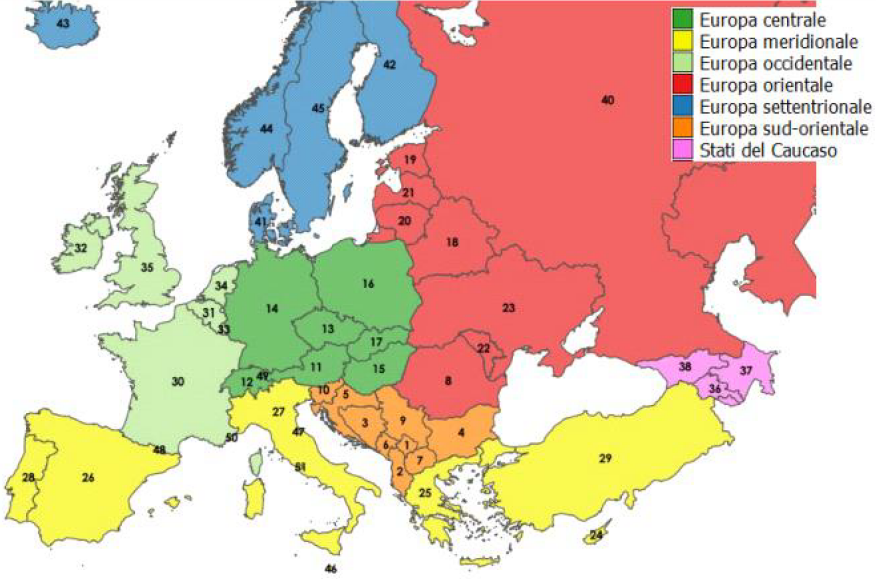
\includegraphics[width=\textwidth]{media/geo_eu/regioni.png}
    \end{center}
\end{figure*}

\subsection{Regioni climatiche}
\setlength{\intextsep}{0pt}%
\begin{wrapfigure}{l}{.5\textwidth}
    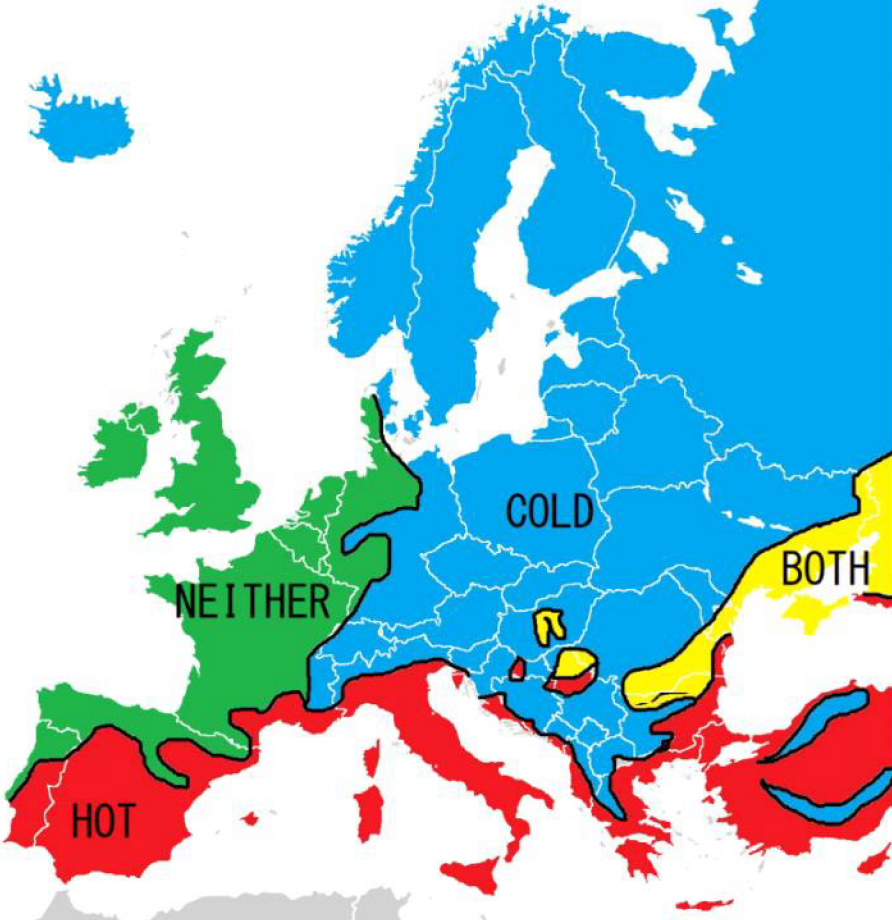
\includegraphics[width=.5\textwidth]{media/geo_eu/clima.png}
    \vspace{-2.1cm}
\end{wrapfigure}

\textbf{Zone climatiche:}
\begin{itemize}
    \item Calde (HOT): aree influenzate dalla latitudine, che incide
        sull'inclinazione dei raggi solari;
    \item Fredde (COLD): aree con condizioni climatiche fredde, sempre
        influenzate dall'inclinazione dei raggi solari;
    \item Né calde né frede (NEITHER): aree influenzate dalle correnti del Golfo
        e dalla vicinanza a grandi masse d'acqua;
    \item Entrambe (BOTH): aree che mostrano caratteristiche sia di
        continentalità che di presenza di catene montuose. 
\end{itemize}
\wrapfill









\end{document}